\documentclass[aspectratio=169, 10pt]{beamer}

% --- Theme & Styling ---
\usetheme{metropolis}
\usepackage{booktabs}
\usepackage{xspace}
\usepackage{tikz}
\usetikzlibrary{arrows.meta, positioning, shapes.geometric, calc}
\usepackage{listings}
\usepackage{tcolorbox}
\usepackage{graphicx}
\usepackage{caption}

% Caption styling for epigraphs below figures
\captionsetup{font=scriptsize, labelfont=bf, textfont=it, skip=2pt, justification=centering}

% --- Color Palette ---
\definecolor{NavyDark}{HTML}{0F172A}
\definecolor{PrimaryBlue}{HTML}{1D4ED8}
\definecolor{TealDark}{HTML}{0F766E}
\definecolor{AmberWarm}{HTML}{B45309}
\definecolor{BgSlate}{HTML}{F8FAFC}
\definecolor{CodeSlate}{HTML}{1E293B}

\setbeamercolor{normal text}{fg=NavyDark, bg=white}
\setbeamercolor{alerted text}{fg=AmberWarm}
\setbeamercolor{example text}{fg=TealDark}
\setbeamercolor{progress bar}{fg=PrimaryBlue, bg=gray!25}
\setbeamercolor{title separator}{fg=PrimaryBlue}
\setbeamercolor{frametitle}{bg=NavyDark, fg=white}

% Metropolis tuning
\metroset{progressbar=frametitle, block=fill}

% Custom image frame styling for screenshots (Option 1: Minimalist Technical Outline)
\newtcbox{\imageframe}{
    colback=NavyDark,
    colframe=NavyDark!40!gray,
    arc=0mm,
    boxrule=0.6pt,
    left=1pt,
    right=1pt,
    top=1pt,
    bottom=1pt,
    boxsep=0pt,
    nobeforeafter
}

% --- Title Information ---
\title{Lab 3: Physical Coding Sublayer (PCS) 64b/66b Encoding \& Scrambling}
\subtitle{Hardware-in-the-Loop Simulation, Self-Synchronizing LFSR \& 66-Bit Waveform Analysis}
\date{\today}
\author{Zuñiga, Ivan Andrés}
\institute{Fundación Fulgor}

\begin{document}

% ==========================================
% SLIDE 1: Title Slide
% ==========================================
\maketitle

% ==========================================
% SLIDE 2: Testbench Architecture & Pipeline
% ==========================================
\begin{frame}{1. System Architecture \& 64b/66b PCS Datapath}
\vspace{1mm}
\begin{columns}[c]
    \begin{column}{0.48\textwidth}
        \textbf{Hardware-in-the-Loop Setup:}
        \begin{itemize}\small
            \item \textbf{Host Interface}: \texttt{tap0} (\texttt{10.0.0.1/24}, MAC \texttt{02:00:00:00:00:01}).
            \item \textbf{Target Interface}: \texttt{tap1} in namespace \texttt{ns\_b} (\texttt{10.0.0.2/24}, MAC \texttt{02:00:00:00:00:02}).
            \item \textbf{RTL Stack (\texttt{top.sv})}: MAC TX/RX, 64b/66b PCS encoder/decoder, and 58-bit parallel LFSR scrambler.
            \item \textbf{C++ Driver (\texttt{wrapper.cpp})}: Non-blocking TAP driver with synchronous clocking across dual Linux namespaces.
            \item \textbf{Specification}: IEEE 802.3 Clause 82 (40G/100GBASE-R).
        \end{itemize}
    \end{column}
    
    \begin{column}{0.50\textwidth}
        \begin{tcolorbox}[colback=BgSlate, colframe=PrimaryBlue, title=\footnotesize IEEE 802.3 Clause 82 PCS Architecture, arc=2mm, top=1.5mm, bottom=1.5mm]
            \centering
            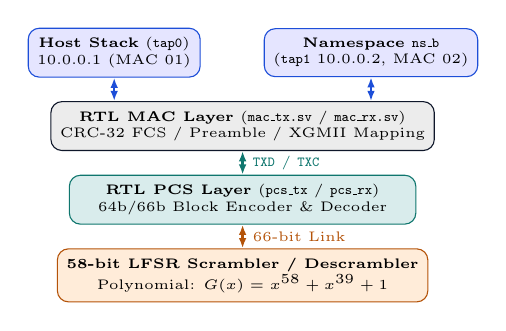
\begin{tikzpicture}[node distance=0.5cm, every node/.style={font=\tiny, align=center}]
                \node[draw=PrimaryBlue, fill=blue!10, rounded corners, minimum width=2.0cm, minimum height=0.55cm] (host) {\textbf{Host Stack} (\texttt{tap0})\\10.0.0.1 (MAC 01)};
                \node[draw=PrimaryBlue, fill=blue!10, rounded corners, minimum width=2.0cm, minimum height=0.55cm, right=0.8cm of host] (nsb) {\textbf{Namespace \texttt{ns\_b}}\\(\texttt{tap1} 10.0.0.2, MAC 02)};
                
                \node[draw=NavyDark, fill=gray!15, rounded corners, minimum width=4.4cm, minimum height=0.55cm, below=0.3cm of $(host.south)!0.5!(nsb.south)$] (mac) {\textbf{RTL MAC Layer} (\texttt{mac\_tx.sv} / \texttt{mac\_rx.sv})\\CRC-32 FCS / Preamble / XGMII Mapping};
                
                \node[draw=TealDark, fill=teal!15, rounded corners, minimum width=4.4cm, minimum height=0.55cm, below=0.3cm of mac] (pcs) {\textbf{RTL PCS Layer} (\texttt{pcs\_tx} / \texttt{pcs\_rx})\\64b/66b Block Encoder \& Decoder};
                
                \node[draw=AmberWarm, fill=orange!15, rounded corners, minimum width=4.4cm, minimum height=0.55cm, below=0.3cm of pcs] (scram) {\textbf{58-bit LFSR Scrambler / Descrambler}\\Polynomial: $G(x) = x^{58} + x^{39} + 1$};
                
                % Arrows
                \draw[{Latex[length=1.3mm]}-{Latex[length=1.3mm]}, thick, color=PrimaryBlue] (host) -- (host |- mac.north);
                \draw[{Latex[length=1.3mm]}-{Latex[length=1.3mm]}, thick, color=PrimaryBlue] (nsb) -- (nsb |- mac.north);
                \draw[{Latex[length=1.3mm]}-{Latex[length=1.3mm]}, thick, color=TealDark] (mac) -- node[right, font=\tiny]{\texttt{TXD} / \texttt{TXC}} (pcs);
                \draw[{Latex[length=1.3mm]}-{Latex[length=1.3mm]}, thick, color=AmberWarm] (pcs) -- node[right, font=\tiny]{66-bit Link} (scram);
            \end{tikzpicture}
        \end{tcolorbox}
        \vspace{1mm}
        \captionof{figure}{Hardware pipeline from Linux TAP devices to the 66-bit physical link.}
    \end{column}
\end{columns}
\end{frame}

% ==========================================
% SLIDE 3: Environment Setup & Traffic Generation
% ==========================================
\begin{frame}{2. Environment Setup \& Traffic Generation}
\vspace{1mm}
\begin{columns}[c]
    \begin{column}{0.48\textwidth}
        \textbf{Execution Sequence:}
        \begin{enumerate}\footnotesize
            \item \textbf{Configure TAP Interfaces}:\\
            \texttt{sudo ./setup\_tap.sh}\\
            {\scriptsize Configures \texttt{tap0} and namespace \texttt{ns\_b} with \texttt{tap1}.}
            
            \item \textbf{Build and Run Verilator Emulator}:\\
            {\scriptsize\texttt{verilator --cc --trace --exe --build wrapper.cpp top.sv}}\\
            \texttt{sudo ./obj\_dir/emulator --enable-scrambler}
            
            \item \textbf{Capture Traffic}:\\
            \texttt{sudo tcpdump -i tap0 -w lab3\_capture.pcap}
            
            \item \textbf{Send Patterned Ping}:\\
            \texttt{ping -c 2 -p cafe0003 -I tap0 10.0.0.2}
        \end{enumerate}
    \end{column}
    
    \begin{column}{0.50\textwidth}
        \centering
        \imageframe{
\includegraphics[width=0.96\linewidth, height=0.64\textheight, keepaspectratio]{figures/screenshot1_terminal.png}}
        \vspace{1mm}
        \captionof{figure}{Terminal execution showing TAP binding, Verilator build, and no packet loss.}
    \end{column}
\end{columns}
\end{frame}

% ==========================================
% SLIDE 4: Wireshark Packet Inspection
% ==========================================
\begin{frame}{3. Layer 2 / Layer 3 Wireshark Packet Analysis}
    \vspace{1mm}
    \textbf{Captured ICMP Echo Request Frame (98 Bytes Total):}
    \begin{itemize}\scriptsize
        \item \textbf{Layer 2 Header (14B)}: Dst MAC \texttt{02:00:00:00:00:02}, Src MAC \texttt{02:00:00:00:00:01}, EtherType \texttt{0x0800} (IPv4).
        \item \textbf{Layer 3 Header (28B)}: IPv4 \texttt{10.0.0.1} $\rightarrow$ \texttt{10.0.0.2} (20B, Len 84B, ID \texttt{0x7F6D}), ICMP Type 8 (Echo Request, Code 0, Checksum \texttt{0xDB80}, ID \texttt{0x7602}, Seq 1).
        \item \textbf{Payload (56B)}: 16-byte kernel timestamp + 40-byte repeating pattern \texttt{ca fe 00 03}.
    \end{itemize}
    
    \vspace{1mm}
    \begin{center}
        \imageframe{
\includegraphics[width=0.98\textwidth, height=0.50\textheight, keepaspectratio]{figures/screenshot2_wireshark.png}}
        \vspace{1mm}
        \captionof{figure}{Wireshark packet dissection and correlated hex dumps.}
    \end{center}
\end{frame}

% ==========================================
% SLIDE 5: IPG & Control Block Validation (BTF = 0x1E)
% ==========================================
\begin{frame}{4. Inter-Packet Gap (IPG) \& Control Block Encoding (\texttt{BTF = 0x1E})}
    \vspace{1mm}
    \textbf{Idle Control Block Compression:}
    \begin{itemize}\scriptsize
        \item \textbf{Idle Input}: MAC outputs \texttt{TXD = 0x0707070707070707} with \texttt{TXC = 8'hFF}, meaning all 8 lanes have an control signal.
        \item \textbf{Control Sync Header}: PCS encoder sets \texttt{Sync = 2'b10} (\texttt{raw\_hdr = 2'b10}) for Control Blocks.
        \item \textbf{Payload Compression}: Sets \texttt{BTF = 0x1E} (bits \texttt{[7:0]}) and compresses 8 idle bytes into 7-bit PCS codes (\texttt{raw\_payload = 64'h000000000000001E}).
    \end{itemize}
    
    \vspace{1mm}
    \begin{center}
        \imageframe{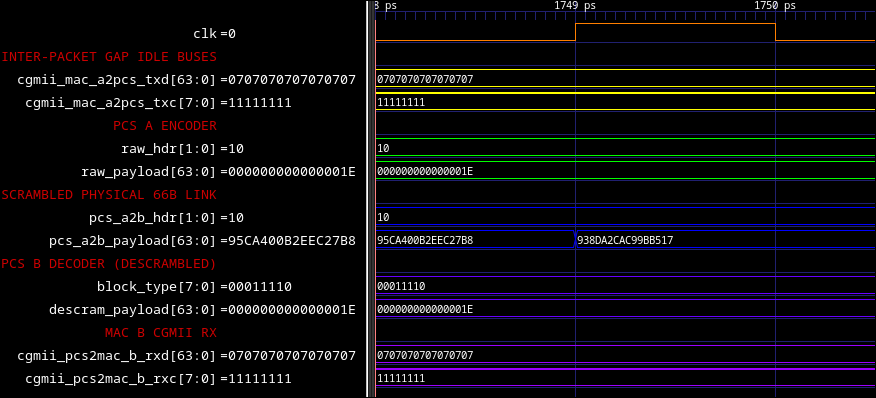
\includegraphics[width=0.94\textwidth, height=0.45\textheight, keepaspectratio]{figures/screenshot3_ipg_idle.png}}
        \vspace{1mm}
        \captionof{figure}{Idle compression: 8 idle bytes encoded into Control Block (\texttt{BTF = 0x1E}, \texttt{Sync = 2'b10}).}
    \end{center}
\end{frame}

% ==========================================
% SLIDE 6: Start Delimiter (/S/) & Control Block (BTF = 0x78)
% ==========================================
\begin{frame}{5. Frame Start Delimiter (\texttt{/S/}) \& Control Block Framing (\texttt{BTF = 0x78})}
    \vspace{1mm}
    \textbf{Frame Start Delimiter \& Block Translation (Cycle 1--2):}
    \begin{itemize}\scriptsize
        \item \textbf{Start Delimiter Detection}: MAC asserts \texttt{/S/ = 0xFB} on Lane 0 with \texttt{TXC = 8'h01} (\texttt{TXD = 0xD5555555555555FB}).
        \item \textbf{Control Block Type 0x78}: PCS encoder outputs \texttt{Sync = 2'b10} and sets \texttt{BTF = 0x78} on Byte 0.
        \item \textbf{Preamble Passing}: Preamble (\texttt{0x55}) and SFD (\texttt{0xD5}) pass into payload bits \texttt{[63:8]} (\texttt{raw\_payload = 0xD555555555555578}).
    \end{itemize}
    
    \vspace{1mm}
    \begin{center}
        \imageframe{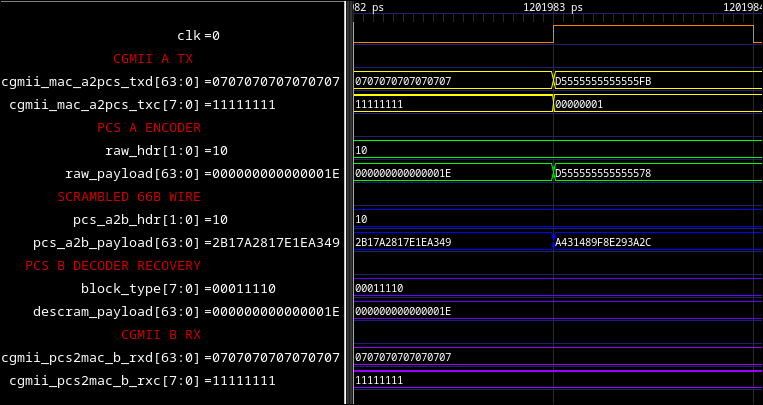
\includegraphics[width=0.94\textwidth, height=0.45\textheight, keepaspectratio]{figures/screenshot4_preamble_start.png}}
        \vspace{1mm}
        \captionof{figure}{Transition from Idle to Frame Start (\texttt{/S/ = 0xFB}) on Lane 0 mapped to \texttt{BTF = 0x78}.}
    \end{center}
\end{frame}

% ==========================================
% SLIDE 7: SW-to-HW Correlation: Data Blocks (Sync = 2'b01)
% ==========================================
\begin{frame}{6. SW-to-HW Correlation: Payload Data Blocks (\texttt{Sync = 2'b01})}
    \vspace{1mm}
    \textbf{64-Bit Data Streaming \& Header Decoding (Cycles 3--12):}
    \begin{itemize}\scriptsize
        \item \textbf{Data Block Framing}: For data words (\texttt{TXC = 8'h00}), PCS encoder sets \texttt{Sync = 2'b01} without BTF overhead.
        \item \textbf{Direct Word Mapping}: Unscrambled payload matches Wireshark byte-for-byte (L2 MACs, IPv4 ID \texttt{0x7F6D}, ICMP Checksum \texttt{0xDB80}).
        \item \textbf{Throughput}: Transmits 8 bytes/cycle at 100\% line rate with 3.125\% framing overhead.
    \end{itemize}
    
    \vspace{1mm}
    \begin{center}
        \imageframe{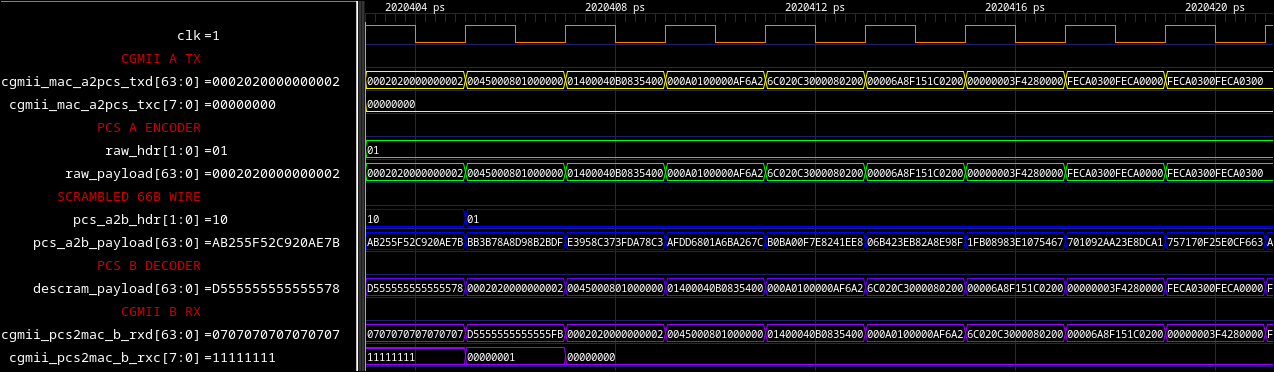
\includegraphics[width=0.94\textwidth, height=0.45\textheight, keepaspectratio]{figures/screenshot5_headers_correlation.png}}
        \vspace{1mm}
        \captionof{figure}{Cycle-by-cycle alignment of L2/L3 packet headers across 64-bit Data Blocks (\texttt{Sync = 2'b01}).}
    \end{center}
\end{frame}

% ==========================================
% SLIDE 8: 58-Bit LFSR Scrambler & Sync Invariance
% ==========================================
\begin{frame}{7. 58-Bit LFSR Scrambler \& Sync Header Invariance}
    \vspace{1mm}
    \textbf{Self-Synchronizing Scrambler Pipeline ($G(x) = x^{58} + x^{39} + 1$):}
    \begin{itemize}\scriptsize
        \item \textbf{Bit Recurrence}: $y[i] = x[i] \oplus y[i - 39] \oplus y[i - 58]$, computed in 1 cycle via self-synchronizing LFSR.
        \item \textbf{Sync Header Invariance}: Sync header \texttt{Sync[1:0]} bypasses the LFSR to preserve receiver block alignment.
        \item \textbf{Descrambler Recovery}: Descrambler recovers payload without sync tokens: $x'[i] = y[i] \oplus y[i - 39] \oplus y[i - 58] \equiv x[i]$.
    \end{itemize}
    
    \vspace{1mm}
    \begin{center}
        \imageframe{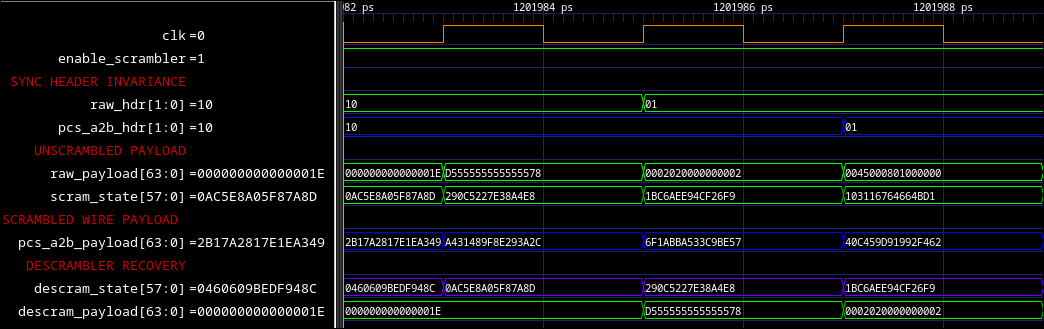
\includegraphics[width=0.94\textwidth, height=0.45\textheight, keepaspectratio]{figures/screenshot6_scrambler_invariance.png}}
        \vspace{1mm}
        \captionof{figure}{Payload bit randomization via $G(x) = x^{58} + x^{39} + 1$ and exact descrambler recovery.}
    \end{center}
\end{frame}

% ==========================================
% SLIDE 9: Mathematical Proof of Self-Synchronization
% ==========================================
\begin{frame}{8. Mathematical Proof of Self-Synchronization}
\vspace{0.5mm}

\textbf{Definitions (IEEE 802.3 Clause 49/82):}
\begin{itemize}\scriptsize
    \item \textbf{Transmitter ($y$)}: Encodes data bit $x[i]$ using past wire bits:
    $$y[i] = x[i] \oplus y[i - 39] \oplus y[i - 58]$$
    \item \textbf{Receiver ($x'$)}: Decodes incoming wire bit $y[i]$ using the same taps:
    $$x'[i] = y[i] \oplus y[i - 39] \oplus y[i - 58]$$
\end{itemize}

\vspace{0.5mm}
\begin{tcolorbox}[colback=BgSlate, colframe=PrimaryBlue, arc=1.5mm, top=1.2mm, bottom=1.2mm, left=3mm, right=3mm]
    \footnotesize\textbf{Algebraic Proof:}
    \vspace{-1.5mm}
    \begin{align*}
        x'[i] &= \underbrace{\big(x[i] \oplus y[i-39] \oplus y[i-58]\big)}_{\text{Substitute } y[i]} \;\oplus\; y[i-39] \;\oplus\; y[i-58] \\[2pt]
              &= x[i] \;\oplus\; \big(y[i-39] \oplus y[i-39]\big) \;\oplus\; \big(y[i-58] \oplus y[i-58]\big) \quad \text{\scriptsize (Associative)} \\[2pt]
              &= x[i] \;\oplus\; 0 \;\oplus\; 0 \quad \text{\scriptsize (Since } A \oplus A = 0\text{\scriptsize)} \\[2pt]
              &\equiv \mathbf{x[i]}
    \end{align*}
\end{tcolorbox}

\vspace{0.5mm}
\textbf{Takeaway:} The receiver recovers clean data with 0 bit errors after 58 bits of wire traffic.
\end{frame}

% ==========================================
% SLIDE 10: Frame Termination (/T/) & BTF Selection (0xE1)
% ==========================================
\begin{frame}{8. Frame Termination (\texttt{/T/}) \& BTF Selection (\texttt{0xE1})}
    \vspace{1mm}
    \textbf{Frame Termination Delimiter \& CRC-32 FCS (Cycle 16):}
    \begin{itemize}\scriptsize
        \item \textbf{CRC-32 FCS}: MAC computes CRC-32 ($P(x) = x^{32}+x^{26}+\dots+1$) over 98 bytes $\rightarrow$ \texttt{0x45210EBC} (Lanes 2--5: \texttt{BC 0E 21 45}).
        \item \textbf{Clause 82 BTF Selection}: Delimiter \texttt{/T/ = 0xFD} on Lane 6 (\texttt{TXC = 8'hC0}) maps to \texttt{BTF = 0xE1} (\texttt{raw\_payload = 0x0045210EBC0300E1}).
        \item \textbf{Hardware Reconstruction}: Decoder detects \texttt{BTF = 0xE1}, restores \texttt{TXC = 8'hC0}, and MAC RX validates the FCS.
    \end{itemize}
    
    \vspace{1mm}
    \begin{center}
        \imageframe{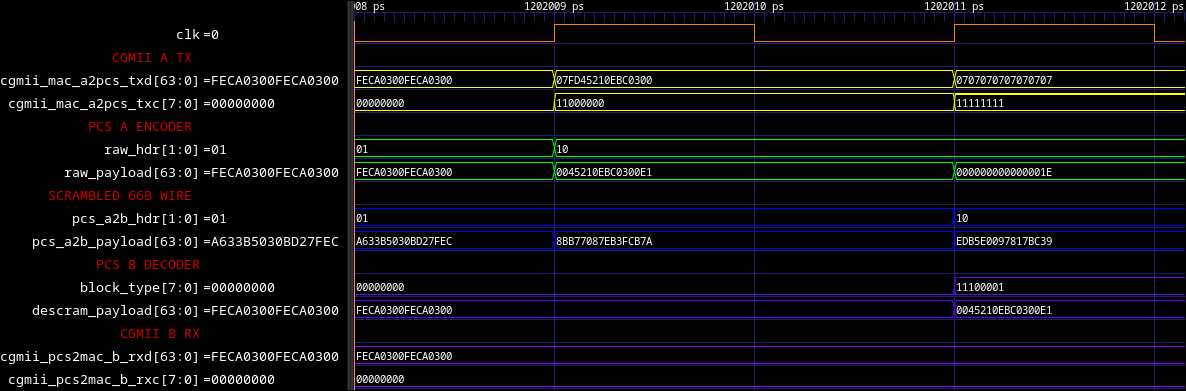
\includegraphics[width=0.94\textwidth, height=0.45\textheight, keepaspectratio]{figures/screenshot7_termination_btf.png}}
        \vspace{1mm}
        \captionof{figure}{Cycle 16 frame termination: \texttt{/T/} on Lane 6 mapped to \texttt{BTF = 0xE1} with CRC-32 FCS (\texttt{0x45210EBC}).}
    \end{center}
\end{frame}

% ==========================================
% SLIDE 11: Conclusion / Standout Slide
% ==========================================
\begin{frame}[standout]
    \Huge \textbf{Thank You!}\\[1.2em]
\end{frame}

\end{document}
